%% History:
%% May 2019 Tomi Männistö, Antti-Pekka Tuovinen proofreading; 30 vs. 40 cr theses, etc.
%% May 2019 Tomi Männistö changed from babelbib to bibtex; Abstract page (and other pages as well) reformatting.
%% January–May 2019 several issues fixed by Niko Mäkitalo; long fields in abstract
%% March 2018 template file extended by Lea Kutvonen to exploit HYthesisML.cls.
%% Feb2018 This template file for the use of HYgraduML.cls was  modified by Veli Mäkinen from HY_fysiikka_LuKtemplate.tex
%% authored by Roope Halonen ja Tomi Vainio in 2017.
%% Some text is also inherited from engl_malli.tex versions by Kutvonen, Erkiö, Mäkelä, Verkamo, Kurhila, and
%% Nykänen, to accompany tktltiki.cls (by Puolakka 2002).


%% Follow comments to support use.

%%%%%%%%%%%%%%%%%%%%%%%%%%%%%%%%%%%%%%%%%%%%%%%%%%%%%%%%%
%% STEP 1: Choose options for MSc / BSc layout and your bibliographic style
%%%%%%%%%%%%%%%%%%%%%%%%%%%%%%%%%%%%%%%%%%%%%%%%%%%%%%%%%

%%  Language: 
%%      finnish, swedish, or english
%%  Pagination (use twoside by default)  
%%      oneside or twoside,
%%  Study programme / kind of report
%%      csm  = pro gradu in new Computer science MSc;
%%      cs = pro gradu in old Computer Science MSc;
%%      tkt = BSc thesis in new curricula;
%%      tktl= BSc thesis in old curricula;
%%  For MSc choose your line or track:
%%      (30 cr thesis, 2020 onwards, Master of Computer Science programme = csm)
%%      software-track-2020 = Software study track
%%      algorithms-track-2020 = Algorithms study track
%%      networking-track-2020 = Networking study track
%%
%%      (30 cr thesis, Master of Computer Science programme = csm)
%%      sw-track-2018 = Software Systems study track
%%      alko-track-2018 = Algorithms study track
%%      nodes-track-2018 = Networking and Services study track
%%
%%      (30 cr thesis, Master of Computer Science programme = csm)
%%      sw-line-2017 =  Software systems subprogramme
%%      alko-line-2017 = Algorithms, Data Analytics and Machine Learning subprogramme
%%      bio-line-2017 = Algorithmic Bioinformatics subprogramme
%%      nodes-line-2017 = Networking and Services subprogramme
%%
%%      (40 cr thesis, = cs)
%%      sw-line = Software Systems specialisation line 
%%      alko-line = Algorithms specialisation line
%%      bio-line = Algorithmic bioinformatics specialisation line
%%      nodes-line = Networking and Services specialisation line

\documentclass[english,twoside,censored,csm,algorithms-track-2020]{HYthesisML}


% In theses, open new chapters only at right page.
% For other types of documents, may ask "openany" in document.
\PassOptionsToClass{openright,twoside,a4paper}{report}
%\PassOptionsToClass{openany,twoside,a4paper}{report}

\usepackage{csquotes}
%%%%%%%%%%%%%%%%%%%%%%%%%%%%%%%%%%%%%%%%%%%%%%%%%%%%%%%%%
%% REFERENCES
%% Some notes on bibliography usage and options:
%% natbib -> you can use, e.g., \citep{} or \parencite{} for (Einstein, 1905); with APA \cite -> Einstein, 1905 without ()
%% maxcitenames=2 -> only 2 author names in text citations, if more -> et al. is used
%% maxbibnames=99 as no great need to suppress the biliography list in a thesis
%% for more information see biblatex package documentation, e.g., from https://ctan.org/pkg/biblatex 

%% Reference style: select one 
%% for APA = Harvard style = authoryear -> (Einstein, 1905) use:
\usepackage[style=authoryear,bibstyle=authoryear,backend=biber,natbib=true,maxnames=99,maxcitenames=2,giveninits=true,uniquename=init]{biblatex}
%% for numeric = Vancouver style -> [1] use:
%\usepackage[style=numeric,bibstyle=numeric,backend=biber,natbib=true,maxbibnames=99,giveninits=true,uniquename=init]{biblatex}
%% for alpahbetic -> [Ein05] use:
%\usepackage[style=alphabetic,bibstyle=alphabetic,backend=biber,natbib=true,maxbibnames=99,giveninits=true,uniquename=init]{biblatex}
%

\addbibresource{bibliography.bib}
% in case you want the final delimiter between authors & -> (Einstein & Zweistein, 1905) 
% \renewcommand{\finalnamedelim}{ \& }
% List the authors in the Bibilipgraphy as Lastname F, Familyname G,
\DeclareNameAlias{sortname}{family-given}
% remove the punctuation between author names in Bibliography 
%\renewcommand{\revsdnamepunct}{ }


%% Block of definitions for fonts and packages for picture management.
%% In some systems, the figure packages may not be happy together.
%% Choose the ones you need.

%\usepackage[utf8]{inputenc} % For UTF8 support, in some systems. Use UTF8 when saving your file.

\usepackage{lmodern}         % Font package, again in some systems.
\usepackage{textcomp}        % Package for special symbols
\usepackage[pdftex]{color, graphicx} % For pdf output and jpg/png graphics
\usepackage{epsfig}
\usepackage{subfigure}
\usepackage[pdftex, plainpages=false]{hyperref} % For hyperlinks and pdf metadata
\usepackage{fancyhdr}        % For nicer page headers
\usepackage{tikz}            % For making vector graphics (hard to learn but powerful)
%\usepackage{wrapfig}        % For nice text-wrapping figures (use at own discretion)
\usepackage{amsmath, amssymb} % For better math

\singlespacing               %line spacing options; normally use single

\fussy
%\sloppy                      % sloppy and fussy commands can be used to avoid overlong text lines
% if you want to see which lines are too long or have too little stuff, comment out the following lines
% \overfullrule=1mm
% to see more info in the detailed log about under/overfull boxes...
% \showboxbreadth=50 
% \showboxdepth=50



%%%%%%%%%%%%%%%%%%%%%%%%%%%%%%%%%%%%%%%%%%%%%%%%%%%%%%%%%
%% STEP 2:
%%%%%%%%%%%%%%%%%%%%%%%%%%%%%%%%%%%%%%%%%%%%%%%%%%%%%%%%%
%% Set up personal information for the title page and the abstract form.
%% Replace parameters with your information.
\title{Weather classification using Convolutional Neural Networks}

% TM: Contributors to template editors now listed in the beginning of the file in comments
\author{Konsta Kutvonen}
\date{\today}



% Set supervisors and examiners, use the titles according to the thesis language
% Prof. 
% Dr. or in Finnish toht. or tri or FT, TkT, Ph.D. or in Swedish... 
\supervisors{Prof. Laura Ruotsalainen}
\examiners{Prof.~D.U.~Mind, Dr.~O.~Why}


\keywords{ulkoasu, tiivistelmä, lähdeluettelo}
\additionalinformation{\translate{\track}}

%% For seminar papers and such, cover page and abstract
%% requires these three basic items of information.
%% Label as needed and remove comment marks.
%%\level{Seminaariraportti}
%%\programme{Tietojenkäsittelytieteen andidaattiohjelma}
%%\subject{Seminaarisarjan nimi}

%% Replace classification terms with the ones that match your work. ACM
%% ACM Digital library provides a taxonomy and a tool for classification
%% in computer science. Use 1-3 paths, and use right arrows between the
%% about three levels in the path; each path requires a new line.

\classification{\protect{\ \\
\  General and reference $\rightarrow$ Document types  $\rightarrow$ Surveys and overviews\  \\
\  Applied computing  $\rightarrow$ Document management and text processing  $\rightarrow$ Document management $\rightarrow$ Text editing
}}

%% if you want to quote someone special. You can comment this line out and there will be nothing on the document.
%\quoting{Bachelor's degrees make pretty good placemats if you get them laminated.}{Jeph Jacques}


%% OPTIONAL STEP: Set up properties and metadata for the pdf file that pdfLaTeX makes.
%% Your name, work title, and keywords are recommended.
\hypersetup{
    unicode=true,           % to show non-Latin characters in Acrobat’s bookmarks
    pdftoolbar=true,        % show Acrobat’s toolbar?
    pdfmenubar=true,        % show Acrobat’s menu?
    pdffitwindow=false,     % window fit to page when opened
    pdfstartview={FitH},    % fits the width of the page to the window
    pdftitle={},            % title
    pdfauthor={},           % author
    pdfsubject={},          % subject of the document
    pdfcreator={},          % creator of the document
    pdfproducer={pdfLaTeX}, % producer of the document
    pdfkeywords={something} {something else}, % list of keywords for
    pdfnewwindow=true,      % links in new window
    colorlinks=true,        % false: boxed links; true: colored links
    linkcolor=black,        % color of internal links
    citecolor=black,        % color of links to bibliography
    filecolor=magenta,      % color of file links
    urlcolor=cyan           % color of external links
}

%%-----------------------------------------------------------------------------------

\begin{document}

% Generate title page.
\maketitle


%%%%%%%%%%%%%%%%%%%%%%%%%%%%%%%%%%%%%%%%%%%%%%%%%%%%%%%%%
%% STEP 3:
%%%%%%%%%%%%%%%%%%%%%%%%%%%%%%%%%%%%%%%%%%%%%%%%%%%%%%%%%
%% Write your abstract to be positioned here.
%% You can make several abstract pages (if you want it in different languages),
%% but you should also then redefine some of the above parameters in the proper
%% language as well, in between the abstract definitions.

\begin{otherlanguage}{english}
\begin{abstract}
Use this otherlanguage environment to write your abstract in another language if needed.

Topics are classified according to the ACM Computing Classification System
(CCS), see 
\url{https://www.acm.org/about-acm/class}:
check command \verb+\classification{}+. A small set of paths (1--3) should be used, starting from any top nodes
referred to bu the root term CCS leading to the leaf nodes. The elements
in the path are separated by right arrow, and emphasis of each element individually can be indicated
by the use of bold face for high importance or italics for intermediate
level. The combination of individual boldface terms may give the reader
additional insight. 
\end{abstract}
\end{otherlanguage}

% Place ToC
\newpage
\mytableofcontents
\frontmatter

%%%%%%%%%%%%%%%%%%%%%%%%%%%%%%%%%%%%%%%%%%%%%%%%%%%%%%%%%
%% STEP 4: Write the thesis.
%%%%%%%%%%%%%%%%%%%%%%%%%%%%%%%%%%%%%%%%%%%%%%%%%%%%%%%%%
%% Your actual text starts here. You shouldn't mess with the code above the line except
%% to change the parameters. Removing the abstract and ToC commands will mess up stuff.
%%
%% You may wish to include material to avoid browsing the definitions
%% above. Command \include{file} includes the file of name file.tex.
%% As a side effect, subsequent inclusions may force a page break.

% BSc instructions
%\include{bsc_finnish_contents}
%
\chapter{Introduction}


In all writing for publication, the writer's freedom of creation and expression are limited by a number of guidelines and specific regulations.

At best, a familiar set of regulations shared by reader and writer can create a kind of support network that allows the message to be relayed without distortion. It will be easier for readers to find 
the pertinent contents in a piece of writing if its layout and structure are the same as they are used to. This also applies to writers. When writers follow a set presentation model, 
they do not have to waste time on considerations that are secondary to the work itself, but they can concentrate on polishing the contents of the text. This means that it is a good 
idea to practice following the rules for the layout, though you may think you know how to select a better way to present your work.

This is a guide for the layout and structure of theses and essays at the Department of Computer Science at the University of Helsinki. It is thus applicable to the course 
Scientific Writing, the software engineering projects, seminars, and MSc theses. (This is an updated version of 
the previous guide written by the course lecturers \citep{erkio01, erkiomakela96, erkio94, verkamo92}.)

The \LaTeX\ guide and \LaTeX\ style that has been  published on the department's web site can be used as support for this guide.


\chapter{Structure}

Let us start by looking at the sections expected to be in a scientific text. Keep in mind that the same expectations go for all kinds of technical writing.
However, this document in itself, is not a scientific or a research
text, so there will be content lacks in terms of research question
setting in the introduction and evaluative material in the last sections.

\section{Abstract or summary}
%\enlargethispage{5mm}


The summary page contains the following elements: the bibliographical data of the work, an abstract, topic classification, 
and the key words. The bibliographical data consists of title, name of the author, place of publication, date of publication, and number of pages.

The abstract should be short, generally one paragraph (100 words maximum) explaining the main contents of the work: topic, methodology and results.


 Topics are classified according to the ACM Computing Classification System
(CCS). A small set of paths (1-3) should be used, starting from any top nodes
referred to bu the root term CCS leading to the leaf nodes. The elements
in the path are separated by right arrow, and emphasis of each element individually can be indicated
by the use of bold face for high importance or italics for intermediate
level. The combination of individual boldface terms may give the reader
additional insight. 

\section{Introduction}


The purpose of the introduction is to introduce the goals of the work in general terms. Describe topic, 
methodology and results (as in the abstract, but expand it).
In order to provide the reader a good starting point for
interpretations, it is good to start the introduction by
contextualisation of the challenges and solutions to be discussed. For
example, why a certain domain has a particular challenge and who are
intended to benefit from the solutions proposed.

The length of the introduction depends on the length of the whole work. A few pages of text does not need a 
separate introduction, since it is an expanded summary in itself. The introduction to a 10-page text can 
be 1--1.5 pages long. For a 50--70-page MSc thesis, a 2--4-page introduction seems reasonable.

The introduction should shortly describe the problem field of the whole work, the plot, and the conclusions, 
in general terms. After reading it, the reader may decide whether to go deeper into the topic by reading the whole text.


\section{Topic chapters}

The nature of the matter at hand determines how the topic chapters are disposed.
In order to guide the reader, it is a good idea to start each main chapter with a short paragraph 
on what the main topic of the chapter is and how it progresses from one sub-chapter to the
next. Especially relevant is to express how concepts, challenges,
solutions and research steps are bound together. There should be enough
guidance for the reader to allow expectation of the right storyline.


Basic rule for easy to follow text is to use the natural emphasis of the
text structure to support the content matter key concepts and thought
processes. This means using openings of sectiosn and text paragraphs for
key arguments and information moves, while the internal parts of
paragraps are filled with supporting aspects that those less familiar
with the topic area need. Those with better background knoweldge can
quickly skim trhough the text without loosing any essential arguments.

Each author has his or her personal ryhtm in the text, which is visible
for the reader as the length of text paragraphs and complexity of
thought chains within. A good policy is to take only one information
move or transition per paragraph. This way the text stays easy to follow.

Signs of problems with the disposition of the text are easily seen in texts
with only one sub-chapter, or with more than two chapter levels (main and sub-chapters). There may be justifiable reasons to use three-level 
headings in some technical documents. Single sentence text paragraphs
are also to be avoided.



%\pagebreak
\section{Reference usage}


Relevant learning targets include superficial knowledge of several
citation styles and capability (and willingness) to follow a given
style and ordering of entires and bibliographical details in the list of references.
These aspects are essential as the approval of a PhD manuscript or
journal article may depend on them.

Disregard of which style you use, 
references are always placed inside sentences.  This means that e.g. a separate reference at the end of a paragraph would be inappropriate.

The structure of the text must clearly show what the reference relates to.  At the same time, it 
shows how long a piece of the text that the reference relates to.

Efficient positions for citations are right after the introduction
(definition) of a concept, a methods or such, or in the end of a claim
from the reference material. Furthermore, if quoting verbatime one must
use citation marks.

The text structures and wordings, in addition to the location of
ciations must clearly express whether claims or arguments are 
authors' own, or if they come from the contribution of others. Thus is
is of bad style to open a section by listing the citations on which the
section is based on. Such method can further indicate more serious
problems like following reference material as it is instead of analysing
and synthetising material into new though processes. 


\section{Conclusion}

At its simplest, a conclusion is merely a weak revision of the main points of the text.  All more valuable 
conclusion sections contain comments on e.g. the value of results, how the work relates to its environment, or 
future visions. This kind of evaluations should be well-grounded in fact, though, or the conclusion 
might inadvertently seem comical. 

\section{Creating the list of references}

The following guidelines should be followed when creating lists of reference for the 
assignments during the course Scientific Writing.

The guidelines are backed by two main goals: to make it as easy as possible to find the 
referenced source, and to show what kind of evaluation process the referenced work has undergone. For these reasons
\begin{itemize}

\item the reference notes should always be so exact that the source can be recognized and found in catalogues and libraries

\item different types of sources (monographs, conferences, journals) have to be easy to distinguish from each other, and 

\item the different parts of the list must conform to each other, especially for each source type.
\end{itemize}


Independent of the citation style in use, 
the sources are listed alphabetically according to the author's name, and works by the same 
author (group of authors) in the order in which they have been published. If some publication 
does not have an individual writer, it is alphabetized according to its name.


The following information should be given on each source independent of
the citation style:
\begin{itemize}
\item
Name(s) of author(s) (surname, initial letters of first names) in the original order; if there are more 
than three authors, we can write the name of the first author and {\em et al.} instead of the other names.

\item
the name of the publication or article in its original form

\item
place of publication:

\begin{itemize}

\item
of monographs: publisher, place of publication (can be omitted if the publisher is well known), year
\item
of journal articles: name of journal, volume, issue, year and month (in parenthesis)

\item
of articles from article collections (such as conference publications):
\begin{itemize}

\item name of collection, editor, publisher, place of publication and year 

{\em or}

\item conference name, coordinator, place and time,

\end{itemize}

\item
of a report: series, report number, place, publisher and year

\item
of a web source: URL, validity date, possibly the date when referenced in square brackets

\end{itemize}

\item
page numbers, if the source is an article or constitutes a chapter in a compilation.
\end{itemize}


When using web sources, you should keep in mind that the threshold for publication on the web 
is non-existent. It is better to concentrate on the publications of well-known scientific 
publishers and the technical standards for which the web is the only publication channel. If 
the same publication is available on paper, refer to that primarily and add the URL as a complement.


The list of references gives an example of a text that has been published through many 
channels~\citep{abiteboul,dietinger}and another example that shows a standard that has 
been disseminated only through the web~\citep{bray}. For web-based
references it is important to give both the publication date and the
time of reading and interpreting the material. The content is prone to
change, and dating your use, you protect your interpretations for
unnecessary accusations of being faulty, if it is known which version
you used.



The list of references for a text should list exactly the sources that the text refers to. 
The list of references for this text is an example of how to present sources, 
which is why it contains ''extra'' sources.


In any style,
put a full stop after the name of a publication or article, as well as after the bibliographical 
data of each reference. Separate the other pieces of information with a comma. As is normal in 
Finnish, only the first letter of the first word in the heading is capitalized, but in the titles of 
conferences and compilations, each major word is capitalized (not articles or prepositions). See the 
appended example for a model. For the sake of clarity, it is best to write {\em In the work} before 
the name of a compilation, except in the case of conference publications where the name starts with 
the abbreviation {\em Proc.} (for Proceedings). In such cases, no complement is necessary. You can 
see the difference by comparing the layouts of the references ~''\citep{dantowsley90}'' and~''\citep{gannonetal89}'' .
In case of other citation styles, it is likely that you can trust the
results given by the automated reference management tools.

\chapter{Layout}

This chapter discusses the main issues of the technical presentation of a text.


\section{Disposition of text sections}


Each text should include a separate cover page, as in this model. The second page contains an 
abstract, followed by a table of contents (on one or more pages), and then the main text.  
Pagination starts on the first page of the main text (with the Arabic numeral 1). (Rigorous writers 
leave out the number from the first page.) All the (numbered) headings and their page numbers should be 
written into the table of contents. Many word-processing systems create the table of contents automatically 
so that the writer does not have to worry about updating page numbers as the work progresses. If writers 
wish to, they can paginate the table of contents and previous pages separately (with Roman numerals), e.g. like this model.

After the main text, but as part of the text body, comes the list of references; its heading is 
not numbered. Any possible appendices are added after the list of references, with headings and internal page numbers.

%\enlargethispage{5mm}

If you want to make a coherent list of figures, algorithms and tables, this list should be placed i
mmediately after the table of contents. The value of such lists is a matter of opinion, so there 
is no need to create one --- especially if your word-processing software does not support it --- unless your instructor explicitly asks for it.

If for some special reason you want to add an alphabetical index top your work, it should be placed after 
the list of references and before appendices. An index should be noted in the table of contents, as s
hould the list of references (unnumbered chapter). Writers who want to create an index should use the automatic support their word-processing system offes.

\section{General text layout}

Nowadays you may plan your text to be printed on single side or double
side, with line spacing one, for the final copy.

For reviewing and feedback purposes, check with your readers for their
preferences. Most read and comment on paper and need some space for
marking. 
For drafts you can use wide margins too. 
Both margins should also be fairly broad (ca.~3~cm): the wider left margin is needed for binding the text and the
right one for the instructor's comments.  Leave enough space (2--3~cm) at the top and bottom, as well.

The most effective way to distinguish features like chapters, figures, etc,  is to have enough space 
in your text.  Separate paragraphs from each other with one and chapters with a few empty lines.  If a 
new chapter is about to start at the bottom of a page (with only one or two lines of text), it is better 
to start it on the next page.  However, it is not necessary to start every chapter on a new page, especially 
not with a short text; if the text contains many pages that are nearly empty, readers might suspect that the 
writer has tried to make it look longer than it is.


Any empty space may be utilized for displaying figures and tables.  Especially if a text is written with the 
same type of text throughout, empty lines are necessary for separating e.g.~text from tables.  Empty space 
is cheap, but adds to the clarity and readability of a text.

\section{Figures and tables}

%\enlargethispage{5mm}

All figures and tables should be placed as near the (first) place in the text that refers to them, but 
not before this reference. The text should also explain what the writer wants to illustrate with the 
figure. Figures can be interpreted in many different ways, so the reader needs guiding.

Figures should never be placed immediately under the heading of a chapter, but chapters should always 
start with text. Figures should not be placed in the middle of a paragraph (much less a sentence), except 
if the figure is placed at the top or bottom of a page and it is clear that the paragraph continues.

Figures do not always have to be placed immediately after the paragraph that refers to them. If there is 
not enough space for a figure on the same page as the paragraph that refers to it, the rest of the page 
should not remain empty, Though the figure is inserted on the following page. However, the figure should 
never be more than one page away from the reference.


The image~\ref{kuvaesimerkki} shows how to present a figure. You must pay attention to the visibility of 
figure parts and text, to the numbering of figures, and captions. 

\begin{figure}[ht]
%\begin{figure}[tbh] t= top, b = bottom, h=here
\ \newline
\begin{center}
\includegraphics[width=0.9\textwidth]{kuvaesimerkki.pdf}
%\rotatebox{90}{\includegraphics[scale=.75]{kuvaesimerkki.pdf}}
\caption{Figure elements.}
\label{kuvaesimerkki}
\end{center}
\end{figure}


We must also pay attention to the size of figures. Any annotations must be clear and easy to read When 
presenting performance curves, for example, the axels have to be named, the scale notated, and the units 
clearly presented. If you present many things with similar figures, you should use the same scale for easy comparison.

The caption of a figure should be written underneath it, and it is preferable that it be short and to 
the point than too explicit. The same goes for table captions.

Figures and tables should be numbered progressively. In long texts, two-level numbering should be 
used (e.g. Figure 3.1) according to the chapter number, but in shorter texts, one-level numbering is good enough.


You should pay attention to presenting figure and table captions consistently, as well as to punctuation 
marks. It is natural to put a full stop after a caption, since they are most often full sentences. 

(The style for figure and table captions vary according to publisher and publication. The recommendations 
at the Department of Computer Science also seems to vary with respect to where the caption should be placed.)


\section{Headings}

You can use a different font in headings than in the rest of the text, or underlining, larger fonts, or other 
methods of emphasis, but generally it is preferred that you only use one of these methods, because if there are 
very many font types and sizes, the layout looks messy.  The format of headings must be consistent throughout 
the text. You should not use any unnumbered ''extra'' headings.


\section{Using this model}

You can use this text as a model for the layout of your own assignment. The font types and sizes, 
line spacing, etc vary according to word-processing system, so small deviations from the rule are acceptable.

The directive number of pages for written assignments given during the lectures for the Scientific-writing 
course and in this guide are applicable to assignments with a layout like this guide's (font size 12 points). The 
average line in this text should consist of about 80~characters and one page about 30~lines. The number of pages 
includes the text itself and the list of references (the part paginated with Arabic numbers), not the 
cover page, summary, or table of contents.

\chapter{Conclusion}

This text is a checklist for some of the rules governing written presentations, which you should 
keep in mind when writing exercises and theses.

This collection of advise has been compiled by staff members as the
result of discussions on general good writing habbits in computer
science. The consensus is that all young researchers and academic degree
holders must be able to seek and follow instructions of layout and
structuring of texts depending on the contribution they are working on. 
This set of instructions aims at unifying the looks of theses and other
study reports from the department, but it is also a representative of
the instruction sets students will meet later.

This set of instructions only address the looks of the document. Other
instructions must be sought, read and gained experience with in order to
learn to select the suitable semantical contents for the scientific texts.

% MSc instructions
%\include{msc_finnish_contents}
\chapter{Introduction}
\section{Problem statement and motivation}
The following gives some superficial instructions for using this template for a Master's thesis. For guidelines on thesis writing you can consult various sources, for example, the Bachelor thesis template.

The thesis should have an introduction chapter. Other chapters can be named according to the topic. In the end, some summary chapter is needed; see Chapter~\ref{chapter:conclusions} for an example.

\section{Structure of thesis}
Cool stuff etc.

\chapter{Neural networks}
Background stuff 
\section{Fully Connected Networks}
When needed, when good/bad
\section{Convolutional Neural Networks}
Show some basic CNN things maybe
\subsection{Neural image processing}
How it different from classical features and how it works
\section{Attention}
Attention huh
\section{Multi-task learning}
Describe how a multi-task setting differs
\section{RNN/LSTM/Transformer text processing/generation}
Depending on what may be used

\chapter{Tasks}
What has been done when solving these tasks/history/formal definition
\section{Image classification}
Image classification is one of the basic modern computer vision problems, where the goal is to create a model that can classify an input image into one of a set of pre-defined classes. Prior to the popularization of applying large Convolutional Neural Networks for this task, the most successful way of solving the problem was to use some algorithm for finding feature descriptors in a set of images and then training a linear classifier, like a Support Vector Machine over a Visual Bag of Words representation of the images. These days nearly all approaches are based on using deep CNNs.
\subsection{ImageNet}
ImageNet  \citep{imagenet}  is perhaps the most significant dataset for image classification and especially the ImageNet Challenge \citep{ILSVRC}, which is a challenge for a collection of 1000 classes from the ImageNet dataset for image classification using 1.2 million training and 150 thousand  images of the entire ImageNet dataset. In 2012 the winning model, AlexNet \citep{alexNet}, showed that it was possible to train a deep CNNs efficiently using GPUs. Since 2012 all top-performing models showed some new improvements on how to create the most performant network architecture, for example, VGGNet from the year 2014 and ResNet \citep{resNet} from 2015, both of which have been popular models to use for Transfer Learning since.

Human accuracy on the ImageNet challenge is about 5.1\% \citep{imageNet_summary}, and ResNet achieves a top-5 error rate of 3.57\% \citep{resNet} and newer architectures even lower, but this still does not mean that image classification is a solved problem. The human performance experiment found that many of the human errors are caused by not having expert information in, for example, identifying animal species or not even being aware of the existence of a class \citep{imageNet_summary}. ObjectNet \citep{objectNet} is a dataset designed to  image classifiers with a focus on their generalizability. It contains many classes that also exist in the ImageNet dataset. However, they are in unexpected locations or have an unexpected pose, causing the high accuracy image classifiers trained on ImageNet experience a 40-45\% accuracy drop when evaluating them on the ObjectNet images of classes shared between ImageNet and ObjectNet. This kind of adjustment is relatively easy for a human, and it shows that while the classifiers are good, they are by no means perfect.
\subsection{Transfer learning}
Unlike the ImageNet challenge, most real-world tasks do not have such an abundance of data for all possible classes. Still, to achieve the highest accuracies, they require models that are equal in terms of complexity to those that have top accuracies problems on the scale of the ImageNet classification. For this reason, many CNN classifiers, irrespective of the problem, feature one of the ImageNet classifiers or similar as a backbone to solve a part of the problem. Even though some datasets may contain a large number of images per class, using a pre-trained classifier as a basis often produces a better final classifier by applying fine-tuning \citep{betterTransfer}.

The idea behind transfer learning is to train on a related task to the end task first. Then the network weights in the model for the actual task are initialized to those of the model we are transferring from, so the training of the original model is a pre-step to the real task. Since training the models on ImageNet scale datasets is not generally feasible due to their large number of parameters and long training time, one of the pre-trained models is picked and then fine-tuned. Fine-tuning a classifier means taking the examples for the final task, and training the network on those, updating the original classifier at the same time. This differs greatly from the traditional learning model where each task is considered to be a separate model that has to be learned from scratch.

\begin{figure}[h!] 
\centering 
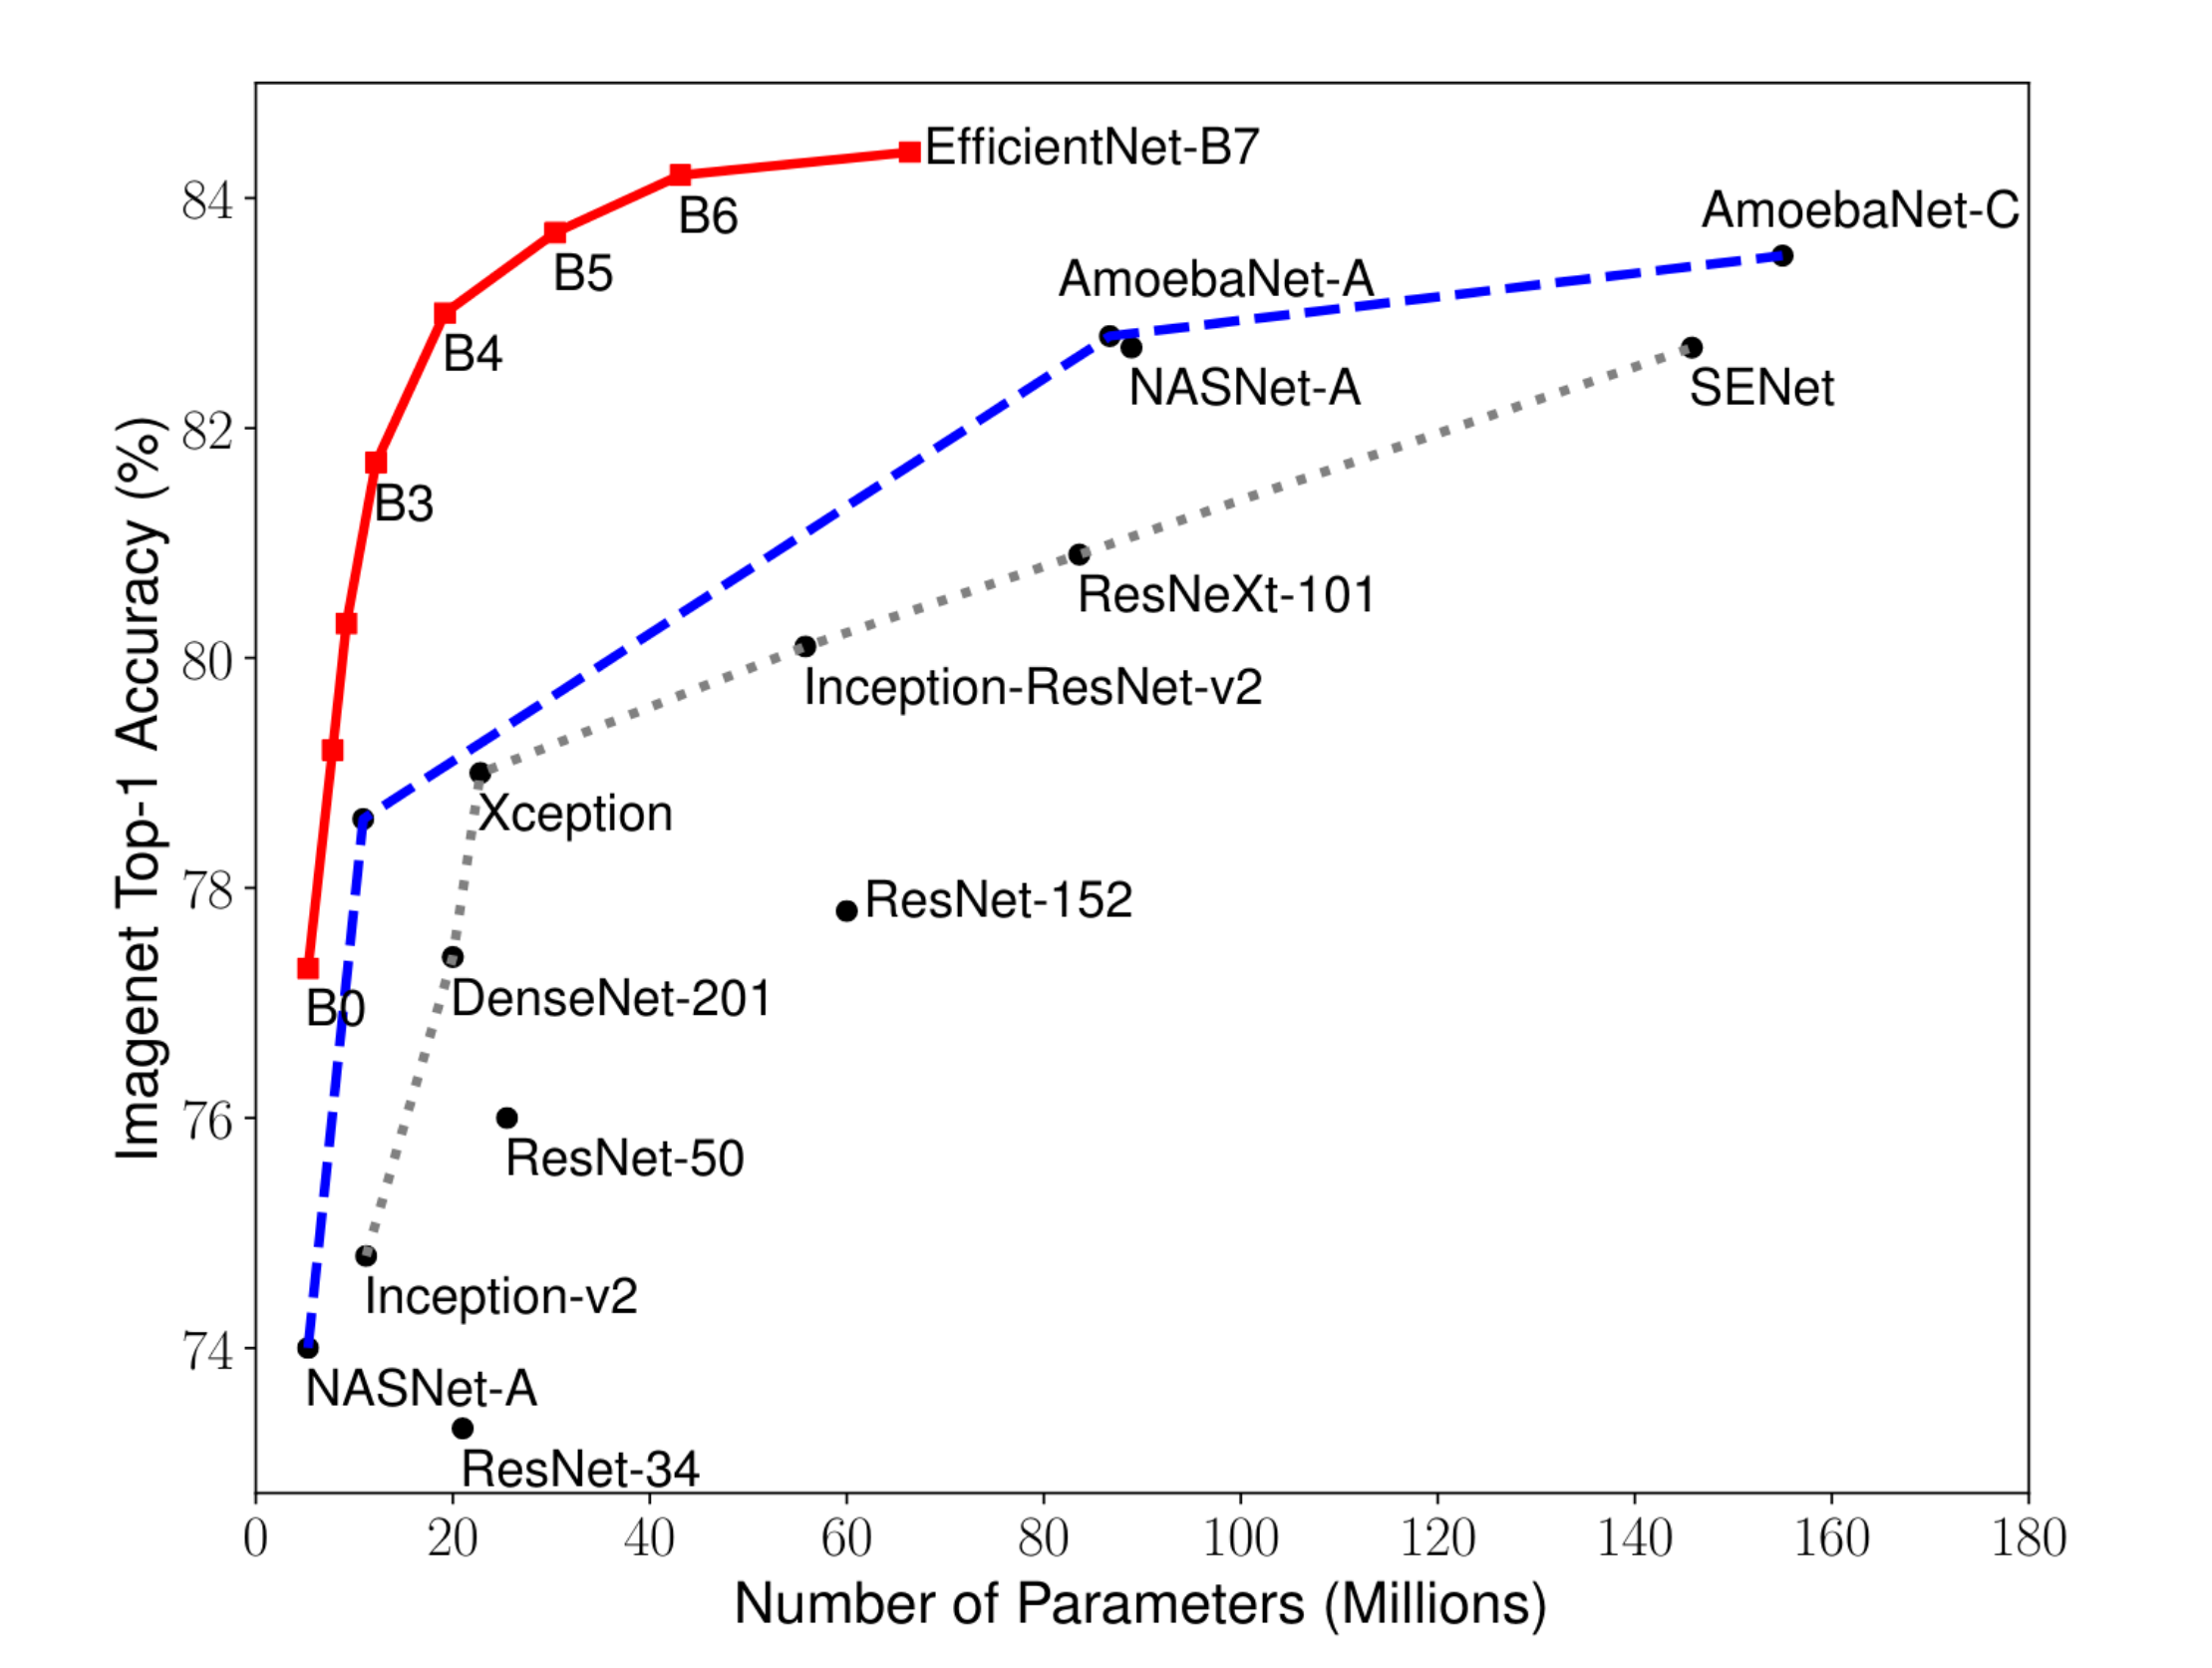
\includegraphics[width=0.8\textwidth]{imgs/imagenet_parameters.png}
\caption{Number of parameters in popular ImageNet classifiers. Figure from \citep{efficientNet}.\label{fig:params}}
\end{figure}

Picking which classifier to use as a base is often problem-dependent. As it is not possible to declare one network structure to be the best at all tasks, picking the best model to start with usually requires the user to compare different architectures and weighing the requirements for the problem at hand. Often though, the larger models will perform better, and there exists a correlation between performing well on ImageNet and being a good transfer learning model \citep{betterTransfer}. Though as can be seen in figure 3.1, better performance often comes at the cost of many more parameters, requiring more memory to train the model. Though just the number of parameters is not the only thing to compare as the throughput of a Resnet50 turns out to be about three times as large as the throughput of an EfficientNet-B4 even though they have a similar amount of parameters \citep{classifierPerformance}.

To formally define transfer learning, let $\mathcal{D}$ be a domain for the features, in this case, images.
\subsection{ResNet}
\subsection{EfficientNet}
\section{Object detection}
Based on what is going to be detected, maybe text?
\section{Paragraph captioning}
Assuming we are doing this
\section{Multi task learning}
Cover some examples of MTL in Computer Vision

\chapter{Datasets}
Describing our data
\section{Data formats}
Describe what datasets are used for each of the tasks and where they are from etc.

\chapter{Experiments}
Here are our experiments
\section{Training process}
\subsection{Evaluation criterias}
eval
\section{Image classifiers}
Results of image classsifiers on the datasets maybe compare ResNet vs EfficientNet
\subsection{Only transfer learned classifier}
Just a ResNet or something
\subsection{Image classifier with attention}
Add attention to image classifier
\subsection{Classifiers combined to a multi-task model}
How it do
\section{Object detection}
Some stuff for object detection
\section{Multi-task models}
Create multi-task models for all and try to find some pairs/tuples that actually work together properly
\chapter{Result analysis}
Incredible models absolutely.

\chapter{Future work}
How to make it better what could be tried 

\chapter{Figures and Tables}

\section{Figures}
Figure~\ref{fig:logo} gives an example how to add figures to the document. Remember always to cite the figure in the main text.

\begin{figure}[h!] 
\centering 

\includegraphics[width=0.3\textwidth]{HY-logo-ml.png}
\caption{University of Helsinki flame-logo for Faculty of Science.\label{fig:logo}}
\end{figure}

\section{Tables}

Table~\ref{table:results} gives an example how to report experimental results. Remember always to cite the table in the main text. 

\begin{table}
\centering
\caption{Experimental results.\label{table:results}}
\begin{tabular}{l||l c r} 
Experiment & 1 & 2 & 3 \\ 
\hline \hline 
$A$ & 2.5 & 4.7 & -11 \\
$B$ & 8.0 & -3.7 & 12.6 \\
$A+B$ & 10.5 & 1.0 & 1.6 \\
\hline
%
\end{tabular}
\end{table}

\chapter{Citations}

\section{Citations to literature}

References are listed in a separate .bib-file. In this case it is named \texttt{bibliography.bib} including the following content:
\begin{verbatim}
@article{einstein,
    author =       "Albert Einstein",
    title =        "{Zur Elektrodynamik bewegter K{\"o}rper}. ({German})
        [{On} the electrodynamics of moving bodies]",
    journal =      "Annalen der Physik",
    volume =       "322",
    number =       "10",
    pages =        "891--921",
    year =         "1905",
    DOI =          "http://dx.doi.org/10.1002/andp.19053221004"
}
 
@book{latexcompanion,
    author    = "Michel Goossens and Frank Mittelbach and Alexander Samarin",
    title     = "The \LaTeX\ Companion",
    year      = "1993",
    publisher = "Addison-Wesley",
    address   = "Reading, Massachusetts"
}
 
@misc{knuthwebsite,
    author    = "Donald Knuth",
    title     = "Knuth: Computers and Typesetting",
    url       = "http://www-cs-faculty.stanford.edu/%7Eknuth/abcde.html"
}
1
\end{verbatim}

In the last reference url field the code \verb+%7E+ will translate into \verb+~+ once clicked in the final pdf.

References are created using command \texttt{\textbackslash cite\{einstein\}}, showing as \citep{einstein}. Other examples: \citep{latexcompanion,knuthwebsite}.

Citation style can be negotiated with the supervisor. See some options in \url{https://www.sharelatex.com/learn/Bibtex_bibliography_styles}.

\section{Crossreferences}

Appendix~\ref{appendix:model} on page~\pageref{appendix:model} contains some additional material.

\chapter{From tex to pdf}

In Linux, run \texttt{pdflatex filename.tex} and \texttt{bibtex filename.tex} repeatedly until no more warnings are shown. This process can be automised using make-command.
 
\chapter{Conclusions\label{chapter:conclusions}}

It is good to conclude with a summary of findings. You can also use separate chapter for discussion and future work. These details you can negotiate with your supervisor.

%%%%%%%%%%%%%%%%%%%%%%%%%%%%%%%%%%%%%%%%%%%%%%%%%%%%%%%%%
\cleardoublepage                          %fixes the position of bibliography in bookmarks
\phantomsection
\addcontentsline{toc}{chapter}{\bibname}  % This lines adds the bibliography to the ToC
\printbibliography

%%%%%%%%%%%%%%%%%%%%%%%%%%%%%%%%%%%%%%%%%%%%%%%%%%%%%%%%%
\backmatter
\begin{appendices}

%
\appendix{Template instructions}


In the HY-CS-main.tex file you will find the following STEPS 0--5. Bellow instructions what each STEP means and how to set up your thesis by following these STEPS.
\vspace{0.5cm}

\textbf{STEP 0 -- Clone the thesis template}

\begin{itemize}
\item One template for all thesis types: \url{https://www.overleaf.com/read/hzgngkgshqwh}
\end{itemize}


{\textbf{STEP 1 -- BSc or MSc thesis?}}
\begin{enumerate}
\item Select whether your are writing BSc (tkt for new, tktl for old) or MSc (csm for new, cs for old, dsm for data science) thesis.
\item Select your language: finnish, english, or swedish.
\item If you are writing MSc select your line / track.
\end{enumerate}


{\textbf{STEP 2 -- Set up your personal information}}

\begin{enumerate}
\item Write the working title of your thesis.
\item Write your name to the author field.
\item Write the names of your supervisors and examiners of the thesis.
\end{enumerate}

{\textbf{STEP 3 -- Write your abstract here}}

\begin{itemize}
\item You can also have the abstract in multiple languages with otherlanguages-environment. Bellow example how to add an english abstract to a thesis written in some other language than english: 

\begin{verbatim}
\begin{otherlanguage}{english} 
\begin{abstract}
Your abstract text goes here. 
\end{abstract} 
\end{otherlanguage}
\end{verbatim}

\end{itemize}

{\textbf{STEP 4 -- Writing your thesis}}

\begin{enumerate}
\item There are some writing instructions in [bsc/msc]\_[finnish/english]\_contents.tex files.
\item You can delete the contents of [bsc/msc]\_[finnish/english]\_contents.tex file and write your thesis inside that file.
\end{enumerate}

{\textbf{STEP 5 -- Set your bibliography style}}

\begin{itemize}
\item The default is Numbering alphabetic order, which should be used in most cases.
\end{itemize}


\appendix{Sample Appendix\label{appendix:model}}
usually starts on its own page, with the name and number of the appendix at the top. 
The appendices here are just models of the table of contents and the presentation. Each appendix
Each appendix is paginated separately.

In addition to complementing the main document, each appendix is also its own, independent entity.
This means that an appendix cannot be just an image or a piece of programming, but the appendix must explain its contents and meaning.

\end{appendices}
%%%%%%%%%%%%%%%%%%%%%%%%%%%%%%%%%%%%%%%%%%%%%%%%%%%%%%%%%

\end{document}
